\chapter{Implementasi dan Pengujian}
\label{chap:implementasi_pengujian}

\section{Implementasi}
\label{chap:implementasi}

\subsection{Lingkungan Implementasi}

Implementasi dilakukan di dua buah mesin. Implementasi pertama dilakukan pada komputer peneliti untuk keperluan pengujian fungsional. Komputer tersebut memiliki spesifikasi seperti berikut:

\begin{itemize}
	\item Prosesor: 1.80 GHz
	\item RAM: 4.00 GB
	\item Sistem Operasi: Windows 8.1 Pro (64-bit)
	\item Versi Java: 1.7.0\_51 (Oracle)
\end{itemize}

Implementasi kedua dilakukan pada sebuah mesin virtual yang dibuat pada \textit{platform Windows Azure} untuk keperluan pengujian eksperimental. Mesin virtual ini terhubung ke internet serta beroperasi 24 jam sehingga dapat melayani permintaan tanpa henti. Adapun spesifikasi dari mesin virtual ini adalah sebagai berikut:

\begin{itemize}
	\item Prosesor: 1 core
	\item RAM: 1.75 GB
	\item Hard disk: 28.8 GB
	\item Sistem Operasi: Ubuntu 14.04.2 LTS (64-bit)
	\item Versi Java: 1.7.0\_79 (OpenJDK)
\end{itemize}

\subsection{Basis Data}

Aplikasi yang dibuat membutuhkan adanya implementasi tabel sesuai dengan yang dijabarkan di tabel \ref{tab:2_struktur_tabel_tracks}. Dalam penelitian ini, digunakan basis data MySQL\footnote{\url{https://www.mysql.com/}}. Dalam pengujian eksperimental, aplikasi menggunakan tabel yang sudah ada di basis data KIRI (bersifat rahasia). Untuk pengujian fungsional, tabel baru akan dibuat dengan beberapa data sampel untuk keperluan pengujian saja. Berikut adalah skrip SQL yang digunakan untuk membentuk dan mengisi tabel tersebut:

\begin{lstlisting}
DROP TABLE IF EXISTS `tracks`;
CREATE TABLE IF NOT EXISTS `tracks` (
	`trackId` varchar(32) NOT NULL,
	`trackTypeId` varchar(32) NOT NULL DEFAULT 'bdo_angkot',
	`trackName` varchar(64) NOT NULL,
	`internalInfo` varchar(1024) NOT NULL,
	`geodata` linestring DEFAULT NULL,
	`pathloop` tinyint(1) NOT NULL DEFAULT '0',
	`penalty` decimal(4,2) NOT NULL DEFAULT '1.00',
	`transferNodes` varchar(1024) DEFAULT NULL,
	`extraParameters` varchar(256) DEFAULT NULL,
	`officialTrackNo` varchar(32) DEFAULT NULL,
	`officialTrackName` varchar(256) DEFAULT NULL
) ENGINE=InnoDB DEFAULT CHARSET=latin1;

INSERT INTO `tracks` VALUES ('testblank', 'bdo_angkot', 'Test Update from NULL', 'angkotwebid:642', GeomFromText(NULL), '0', '1.00', NULL, NULL, '1A', 'Abdul Muis - Cicaheum (via Binong)');
\end{lstlisting}

\section{Hasil Pengujian}

\subsection{Pengujian Fungsional}

TODO

\subsection{Pengujian Eksperimental}

Pengujian eksperimental dibagi menjadi 3 tahap:

\begin{enumerate}
	\item Survei \textit{online} terhadap kepuasan kualitas pencarian pengguna, dan potensi keinginan untuk berkontribusi selama satu bulan.
	\item Kampanye fitur integrasi perbaikan rute.
	\item Survei \textit{online} terhadap kepuasan kualitas pencarian serta keterlibatan pengguna dalam perbaikan rute.
\end{enumerate}

Ketiga tahap tersebut dijelaskan pada subbab-subbab berikut.

\subsubsection{Tahap 1: Survei Kepuasan Kualitas Pencarian dan Potensi Keinginan Berkontribusi}

Pada tahap ini, peneliti membuat survei \textit{online} memanfaatkan aplikasi Google Docs\footnote{\url{https://google.com/docs}}. Ada 6 pertanyaan yang ditanyakan, yaitu:

\begin{itemize}
	\item \textbf{Seberapa baik rute kami secara keseluruhan?} (mengerikan / buruk / netral / baik / sempurna)
	\item \textbf{Seberapa baik rute kami pada bagian rute kendaraan?} (mengerikan / buruk / netral / baik / sempurna)
	\item \textbf{Seberapa baik rute kami pada bagian rute berjalan?} (mengerikan / buruk / netral / baik / sempurna)
	\item \textbf{Di kota apa Anda menggunakan KIRI?} (Bandung / Jakarta / Malang / Surabaya)
	\item \textbf{Di mana Anda tinggal?} (Bandung / Jakarta / Malang / Surabaya)
	\item \textbf{Apakah Anda tertarik untuk berkontribusi data rute?} (Ya, dengan imbalan / Ya, tanpa syarat / Tidak / Tidak tahu)
\end{itemize}

Survei ini disediakan \textit{online} pada alamat \url{http://goo.gl/forms/WkeU8oK4Ek}, dan ditunjukkan pada situs web KIRI setelah hasil pencarian ditampilkan (Gambar \ref{fig:5_survei_1}) selama bulan April 2015.

\begin{figure}
	\centering
	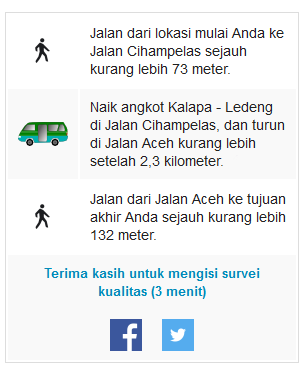
\includegraphics[scale=0.75]{Gambar/5_survei_1}
	\caption{Tautan ke Survei Tahap 1} 
	\label{fig:5_survei_1}
\end{figure}

Setelah masa survei berakhir, didapatkan 33 responden survei. Dari segi kualitas pencarian (Gambar \ref{fig:5_hasilsurvei_1_1}), secara umum pengguna puas dengan hasil kualitas pencarian, ditandai dengan sebagian besar pengguna memilih "baik" pada ketiga jenis pertanyaan. Pada bagian kualitas rute kendaraan, relatif lebih banyak pengguna yang memilih "sempurna" dibandingkan dengan rute berjalan. Peneliti menduga bahwa ini dikarenakan oleh dua hal:

\begin{itemize}
	\item Pencarian rute di KIRI relatif lebih baik dibandingkan dengan pada situs web sejenis\footnote{\url{http://angkot.tibandung.com/}}, karena lebih presisi hingga titik koordinat.
	\item Karena keterbatasan data, hasil rute berjalan di KIRI menghasilkan garis lurus dan tidak mengikuti arah jalan yang sesungguhnya.
\end{itemize}

Dari segi demografi pengguna (Gambar \ref{fig:5_hasilsurvei_1_2}, sebagian besar pengguna menggunakan KIRI di Bandung dan tinggal di Bandung. Hal ini memberikan dua keuntungan kepada peneliti:

\begin{itemize}
	\item Sesuai dengan batasan masalah, yaitu penelitian dilakukan di kota Bandung.
	\item Pengguna relatif mengenal rute transportasi publik di Bandung, karena tinggal di kota Bandung.
\end{itemize}

Terakhir, survei mengenai potensi keinginan berkontribusi (Gambar \ref{fig:5_hasilsurvei_1_3}) memberikan hasil yang bervariasi. Sebagian besar responden bersedia memperbaiki rute yang salah, namun ada juga yang berharap imbalan maupun tidak berminat. Hasil tersebut cukup meyakinkan peneliti bahwa pada tahap berikutnya akan ada sebagian dari pengguna yang bersedia memperbaiki.

\begin{figure}
	\centering
	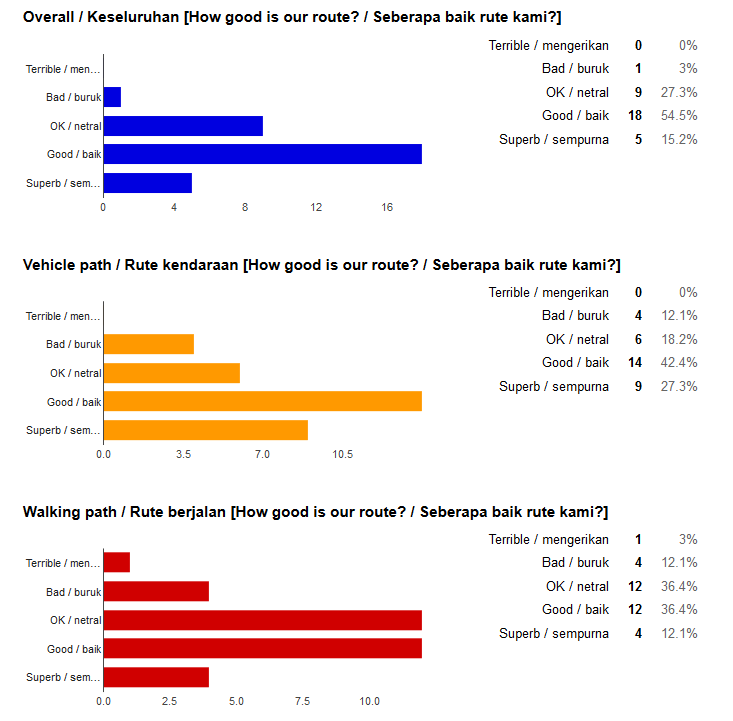
\includegraphics[scale=0.75]{Gambar/5_hasilsurvei_1_1}
	\caption{Hasil Survei Tahap 1 (Kualitas Pencarian)} 
	\label{fig:5_hasilsurvei_1_1}
\end{figure}

\begin{figure}
	\centering
	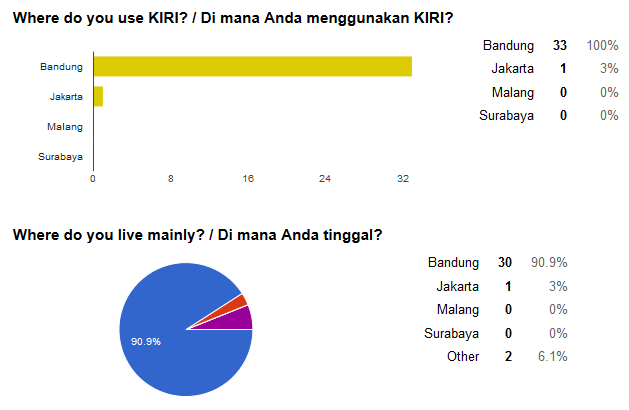
\includegraphics[scale=0.75]{Gambar/5_hasilsurvei_1_2}
	\caption{Hasil Survei Tahap 1 (Demografi Pengguna)} 
	\label{fig:5_hasilsurvei_1_2}
\end{figure}

\begin{figure}
	\centering
	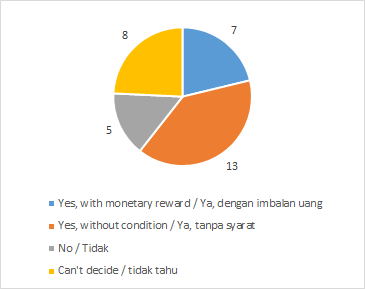
\includegraphics[scale=0.75]{Gambar/5_hasilsurvei_1_3}
	\caption{Hasil Survei Tahap 1 (Kesediaan Berkontribusi)} 
	\label{fig:5_hasilsurvei_1_3}
\end{figure}

\subsubsection{Tahap 2: Kampanye fitur integrasi perbaikan rute}

Setelah fitur integrasi diimplementasikan, KIRI perlu mendorong penggunanya untuk berpartisipasi dalam perbaikan rute. Di situs KIRI sendiri, sebuah tautan akan diberikan setelah hasil pencarian diberikan. Jika tautan tersebut diklik, maka akan membuka video\footnote{\url{https://www.youtube.com/watch?v=jDFePujA8Kk}} di situs \textit{Youtube} yang menunjukkan langkah-langkah dalam memperbaiki rute yang salah di KIRI. Tautan ini terletak di tempat yang sama seperti pada saat survei di tahap 1, dan dapat dilihat pada gambar \ref{fig:5_petunjuk}.

\begin{figure}
	\centering
	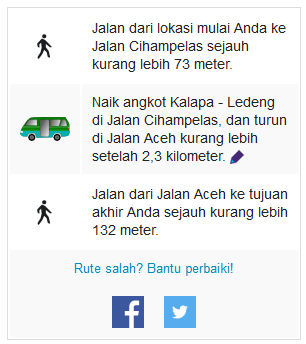
\includegraphics[scale=0.75]{Gambar/5_petunjuk}
	\caption{Tautan ke Petunjuk Perbaikan} 
	\label{fig:5_petunjuk}
\end{figure}

Selain itu, dilakukan juga kampanye berupa iklan di situs media sosial \textit{Facebook}\footnote{\url{https://www.facebook.com/}} selama satu bulan. Parameter-parameter yang digunakan untuk iklan ini adalah sebagai berikut:

\begin{itemize}
	\item Budget, Schedule \& Optimization:
	\begin{itemize}
		\item Budget: Rp 1,500,000 lifetime
		\item Schedule: 06/01/2015 - 06/30/2015
		\item Duration: 29 days
		\item Bidding: Bid for website clicks
		\item Pricing: Your bid will be optimized to get more clicks to your website. You'll be charged each time your ad is served.
	\end{itemize}
	\item Targeting \& Placement:
	\begin{itemize}
		\item Location - Living In: Indonesia / Bandung (+25 mi) West Java
		\item Behaviors: Technology early adopters
		\item Age: 18 - 65+
		\item Language: Indonesian
		\item Mobile Placement: Third-party Apps or News Feed
		\item Desktop: News Feed or Right Column
	\end{itemize}
	\item Estimated Daily Reach: 2,800 - 7,400 peoples
\end{itemize}

Berdasarkan laporan dari \textit{Facebook}, iklan tersebut menghasilkan TODO buah klik.